\RequirePackage{shellesc}
\immediate\write18{tex braids.dtx}
\documentclass{article}

\usepackage{tikz}
\usetikzlibrary{braids}

\begin{document}
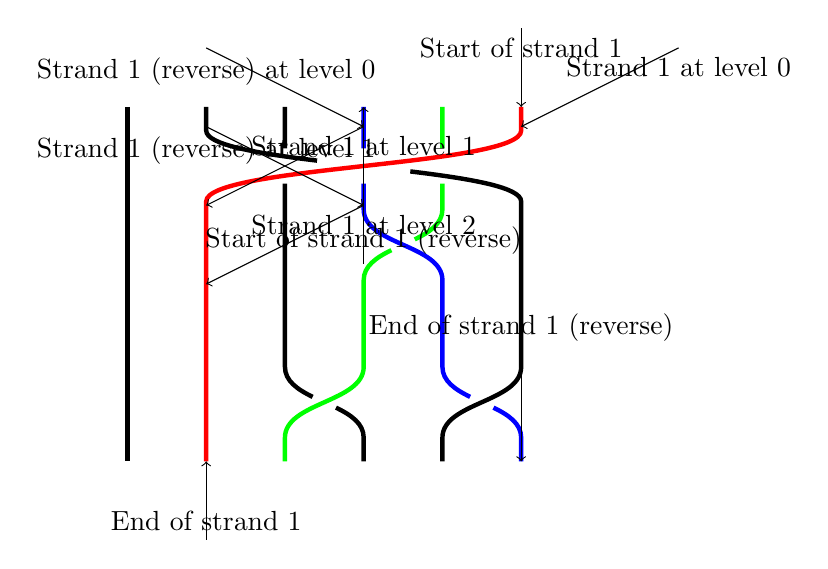
\begin{tikzpicture}
\pic[
  ultra thick,
  braid/strand 1/.style={red},
  braid/strand 2/.style={green},
  braid/strand 3/.style={blue},
  braid/every fence/.style={draw},
  braid/fence 1/.style={fill=yellow,draw=none},
  braid/number of strands=6,
  braid/width=-1cm,
  braid/gap=.1,
  name prefix=braid,
] {braid={| s_{1,5} s_2^{-1} | 1 s_3-s_1}};% s_2 | s_1^{-1}-s_3 | 1 s_1}};
\begin{scope}[yscale=-1]
\draw[<-] (braid-1-e) -- +(0,1) node[above] {End of strand 1};
\draw[<-] (braid-1-s) -- +(0,-1) node[below] {Start of strand 1};
\draw[<-] (braid-rev-1-e) -- +(0,-2) node[below] {End of strand 1 (reverse)};
\draw[<-] (braid-rev-1-s) -- +(0,2) node[above] {Start of strand 1 (reverse)};
\draw[<-] (braid-1-2) -- +(2,-1) node[below] {Strand 1 at level 2};
\draw[<-] (braid-1-1) -- +(2,-1) node[below] {Strand 1 at level 1};
\draw[<-] (braid-rev-1-1) -- +(-2,-1) node[below] {Strand 1 (reverse) at level 1};
\draw[<-] (braid-1-0) -- +(2,-1) node[below] {Strand 1 at level 0};
\draw[<-] (braid-rev-1-0) -- +(-2,-1) node[below] {Strand 1 (reverse) at level 0};
\end{scope}

\end{tikzpicture}
\end{document}
